\documentclass[11pt, aspectratio=169]{beamer}

% --- Core Packages for Modern Documents ---
\usepackage{fontspec}      
\usepackage{unicode-math}
% \usepackage{xeCJK}         
\usepackage{graphicx}      
\usepackage{minted}
\usepackage{setspace}
% \usepackage{tipa}
\usepackage{kotex}
\usepackage{graphicx}
\usepackage{tikz}
\usepackage{multicol}
\usepackage{hyperref}
\usepackage{emoji}

\usetikzlibrary{
    shapes.geometric, % 다양한 도형 사용
    arrows.meta,      % 화살표 스타일 설정
    positioning       % 노드 위치 선정
}

% \xeCJKsetup{CJKspace=true}

% --- Font Setup ---
\setsansfont{Noto Sans KR} %Noto Sans KR
\setmainfont{Noto Serif KR}
\setmonofont{D2Coding}

\setmainhangulfont{Noto Sans KR}
\setsanshangulfont{Noto Serif KR}
\setmonohangulfont{D2Coding}

% \setCJKsansfont{Noto Sans KR}  %나눔바른고딕 옛한글
% \setCJKmainfont{Noto Serif KR}
% \setCJKmonofont{D2Coding}

\setmathfont{Latin Modern Math}

\newfontfamily{\tnrfont}{Times New Roman}
\newcommand{\texttnr}[1]{{\tnrfont #1}}

\mode<presentation>
{
  \usetheme{default}      % or try Darmstadt, Madrid, Warsaw, Marburg...
  \usecolortheme{dove} % or try albatross, beaver, crane, dove...
  \usefonttheme{default}  % or try serif, structurebold, ...
  \setbeamertemplate{navigation symbols}{}
  \setbeamertemplate{caption}[numbered]
} 

\AtBeginSection[]{
  \begin{frame}
    \vfill % Vertically center the title
    \centering
      \usebeamerfont{title}\insertsectionhead\par
    \vfill
  \end{frame}
}

\renewcommand{\arraystretch}{1.3} % Set row height for ALL tables in the document to 1.5x

\definecolor{Highlight}{HTML}{FFF2CC} % A soft yellow

\definecolor{MonokaiBackground}{HTML}{272822}
\definecolor{blocktitle}{HTML}{7A8B5D}
\definecolor{blockbody}{HTML}{F0E085}
\definecolor{normaltext}{HTML}{E5E8D5}
\definecolor{structure_color}{HTML}{D1E1E8}

\setbeamercolor{normal text}{bg=normaltext, fg=black}
\setbeamercolor{structure}{bg=structure_color, fg=black}

\setbeamercolor{block title}{bg=blocktitle, fg=white}
\setbeamercolor{block body}{bg=blockbody, fg=black}
\setbeamertemplate{footline}{
  \hfill % Pushes the content to the right
  \usebeamercolor{page number in head/foot}
  \usebeamerfont{page number in head/foot}
  \insertframenumber{} / \inserttotalframenumber
  \hspace*{2ex} % Adds a little padding from the right edge
}

\setminted{
    style=default, % dracula, native, monokai...
    linenos,       % Show line numbers
    frame=lines,   % Draw a thin frame around the code
    framesep=2mm,
    xleftmargin=6pt,
    breaklines=true
}

% 제목 정보
\title{언어의 이해}
\subtitle{1강. 언어와 언어학: 퀴즈}
\author{김미경}
\date{2025.9.8}

\begin{document}

% 제목 슬라이드
\frame{\titlepage}

\begin{frame}[t]{출결 주의 사항}
    \begin{itemize}
        \item 1주차의 출석은 성적에 반영하지 않습니다. 전원 출석처리 되어 있습니다.
        \item 2주차부터 출석이 성적에 반영됩니다. 전자출결이 제대로 처리되었는지 늘 확인해 주세요. 
        \item 동영상 강의를 시청해도 출석으로 인정되지 않습니다. 강의실에 와 주세요. 
    \end{itemize}
\end{frame}

\begin{frame}[t]{언어와 언어학: 퀴즈}
  \begin{block}{문 1.}
    다음은 조선 전기의 인물인 신숙주에 대한 유튜브 쇼츠 영상에 적혀 있는 소개글입니다. 해당 영상에서는 신숙주가 7개 국어를 구사하는 인물이었다는 점을 소개하고 있습니다. 언어학의 관점에서, 이 소개글에 어떤 문제가 있는지 지적하고 어떻게 정정되어야 하는지 설명하세요.\\
    
\includegraphics[width=1.0\textwidth]{img/linguist_vs_polyglot.png}
  \end{block}
\end{frame}

\begin{frame}[t]{언어와 언어학: 퀴즈}
  \begin{block}{문 2.}
    태희가 철수에게 ‘와 오늘 구름이 가을 구름인데?’라고 말했습니다. 이 때 태희와 철수의 머릿속에서 어떤 일이 일어나는지, 단계를 최대한 자세히 나누어 설명하세요. 
  \end{block}
\end{frame}

\begin{frame}[t]{언어와 언어학: 퀴즈}
  \begin{block}{문 3.}
    우리는 ‘뜨거운 아이스 아메리카노’라는 표현을 들었을 때 그것이 한국어이기는 하지만 이상한 표현이라고 느끼고, 화자가 왜 그런 말을 했는지 의도를 짐작하려고 합니다. 반면에 ‘접시가 어제 잠을 쿨쿨 잘 것이다’라는 표현을 들으면 잘못된 한국어라고 느끼며 어디가 틀렸는지 즉각 지적을 하게 됩니다. 이러한 현상을 토대로, 언어학이 언어의 구조를 어떻게 연구하는지 설명하세요.
  \end{block}
\end{frame}

\begin{frame}[t]{언어와 언어학: 퀴즈}
  \begin{block}{문 4.}
    인간의 언어를 연구하는 연구자들은 사람들이 어떻게 적절한 언어 표현을 만들어내는지, 왜 그것이 적절한 언어 표현으로 받아들여지는지 알아내고 싶어합니다. 그러나 이것을 알기 위해서 연구자들은 사람들에게 ‘어떻게 언어 표현을 만드는지, 왜 그것이 적절한지’ 물어보는 대신, 사람들이 어떤 언어 표현을 만들어내고 어떤 언어 표현을 만들어내지 않는지를 관찰합니다. 언어 연구자들이 언어를 연구할 때 이런 방법을 쓰는 이유는 무엇인지 설명하세요. 
  \end{block}
\end{frame}

\begin{frame}[t]{언어와 언어학: 퀴즈}
  \begin{block}{문 5.}
    다음은 한 논문에 제시된 ‘참조문법(reference grammar)’에 대한 서술입니다. 이 서술을 토대로 ‘참조문법’이 기술문법(descriptive grammar)의 한 종류인지 규범문법(prescriptive grammar)의 한 종류인지 판단하고, 그렇게 생각한 이유를 서술하세요. 
  \end{block}
  {\scriptsize […] 참조문법이란 특정 언어의 주요 문법 구조에 대한 자세한 기술을 시도한 문법서를 말한다. 참조문법은 교육문법과는 달리 한국어 학습에 사용하려는 목적보다는 정보를 제공하기 위한 목적으로 작성된다. 참조문법서는 모어화자를 대상으로 할 수도 있고 해당 언어에 관심이 있는 외국어 화자를 대상으로 할 수 있다. 모어화자는 해당 언어를 사용할 줄 알지만 문법 자체에 대한 인식은 없으므로 참조문법을 통해 모어의 문법적 특징에 대한 기술을 제공할 필요가 있다. 외국어 화자나 언어학자는 일반적인 언어학적 지식을 가지고 있으면서 해당 언어의 문법에 대한 지식을 알고자 하므로 참조문법은 보편적인 언어학적 틀을 기준으로 정보를 제시하게 된다. 본고에서 다루고자 하는 한국어에 대한 참조문법서는 한국어를 연구하거나 한국어의 문법적 특징에 대해 알고자 하는 외국어 화자를 대상으로 한 문법서들이다. […] (이은경 2017:244)\\
  이은경 (2017) ‘참조문법에서의 어말어미 기술에 대하여’, 한국어학 75, 243-272쪽}
\end{frame}

\begin{frame}[t]{언어와 언어학: 퀴즈}
  \begin{block}{문 6.}
    한국어 ‘짜장면’은 1950년대부터 쓰이던 단어이지만 ‘짜장면’이 표준어로 인정된 것은 2011년의 일입니다. 실제로 사람들이 더 많이 쓰는 표현은 ‘짜장면’이었지만, ‘자장면’이 표준어로 인정된 것은 1986년에 국어연구소(현재 국립국어원의 전신)에서 이 단어의 어원은 중국어 炸醬麵(zhajiangmian)이므로 ‘zh'를 ‘ㅈ’으로 쓰는 외래어 표기법에 따라 ‘자장면’으로 써야 다른 중국어 유래 단어들과 일관성을 유지할 수 있다고 보았기 때문입니다. 이 사례에서 드러나는 규범문법의 특징에 대해 설명하세요. 
  \end{block}
\end{frame}

\begin{frame}[t]{언어와 언어학: 퀴즈}
  \begin{block}{문 7.}
    Charles Hockett은 1960년대에 언어가 갖는 특징으로 9가지 성질을 지적했습니다. 이 중에서 7가지는 다른 동물의 의사소통 체계에서 관찰되는 경우가 있지만, 전위성(displacement)과 생산성(productivity)은 인간의 언어에서만 발견되는 것으로 여겨집니다. 이 두 가지 특성이 구체적으로 인간 언어의 어떤 측면을 말하는 것인지 각각 설명하세요. 
  \end{block}
\end{frame}

\begin{frame}[t]{언어와 언어학: 퀴즈}
  \begin{columns}
    \begin{column}{0.6\textwidth}
      \begin{block}{문 8.}
        A는 XYZ라는 게임을 하다가 게임에서 ‘이달의 꽃’이라고 소개된 맨드라미의 이미지가 사람의 뇌와 비슷하다는 생각을 했습니다. 그런 A에게 B가 다음과 같이 물었습니다.
        \begin{itemize}
          \item B: 이번 달 XYZ 꽃이 뭐였지?
          \item A: 뇌.
          \item B: ….
          \item A: …맨드라미, 길어. 뇌. \\ (알아듣기만 하면 되는 거 아닌가…?)
        \end{itemize}
        A와 B의 의사소통이 잘 이루어지지 않은 이유는 무엇인가요? 언어의 ‘자의성(arbitrariness)’을 중심으로 설명하세요.
      \end{block}      
    \end{column}
    \begin{column}{0.33\textwidth}
      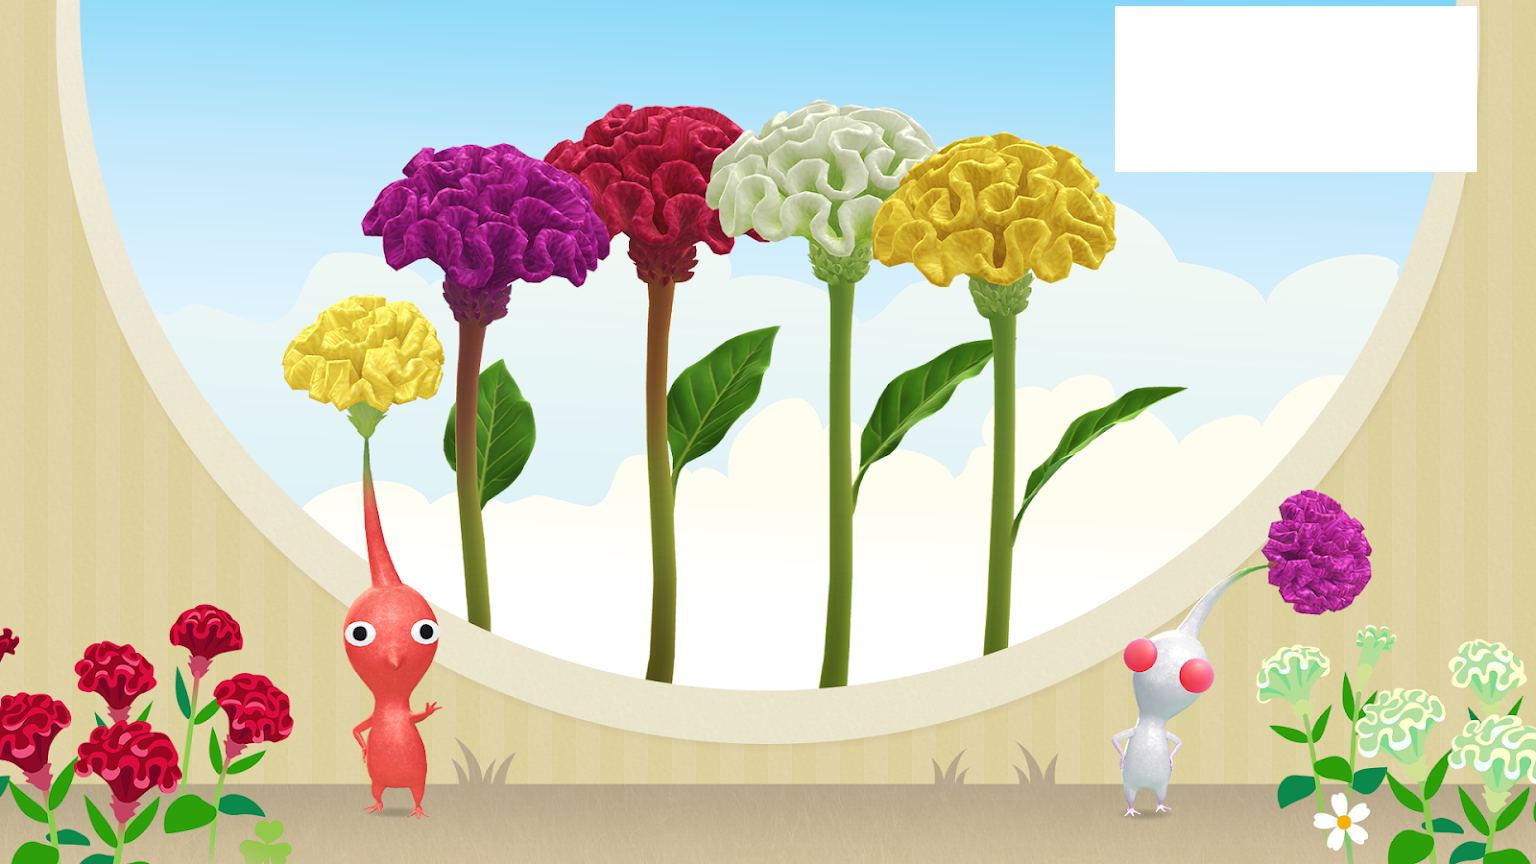
\includegraphics[width=1.5\textwidth]{img/IMG_8059.png}      
    \end{column}
  \end{columns}
\end{frame}

\begin{frame}[t]{언어와 언어학: 퀴즈}
  \begin{block}{문 9.}
    중세 유럽에서 학문을 연구하던 사람들은 그리스어와 라틴어 등 고전어만을 연구할 가치가 있는 언어로 인식했고, 자기들이 일상생활에서 쓰는 모어는 특별히 이름을 붙이거나 연구의 대상으로 삼을 생각을 하지 않았습니다. 이들이 자신들의 모어를 그리스어나 라틴어 등과 마찬가지로 독자적인 체계를 지닌 언어로 인식하게 된 계기에 대해 설명하세요. 
  \end{block}
\end{frame}


\end{document}